\chapter{Overview of Uintah} \label{Sec:Overview} 
The Uintah Computational Framework, (also referred to as Uintah or the UCF)
consists of a set of
software components and libraries that facilitate the solution of
Partial Differential Equations (PDEs) on Structured AMR (SAMR) grids
using hundreds to thousands of processors.

One of the challenges in designing a parallel, component-based
multi-physics application is determining how to efficiently decompose
the problem domain. Components, by definition, make local
decisions. Yet parallel efficiency is only obtained through a globally
optimal domain decomposition and scheduling of computational
tasks. Typical techniques include allocating disjoint sets of
processing resources to each component, or defining a single domain
decomposition that is a compromise between the ideal load balance of
multiple components. However, neither of these techniques will achieve
maximum efficiency for complex multi-physics problems.

Uintah uses a non-traditional approach to achieving parallelism,
employing an abstract taskgraph representation to describe computation
and communication. The taskgraph (for an example, see Figure~\ref{fig:TaskGraph}) is an explicit representation of the
computation and communication that occur in the coarse of a single
iteration of the simulation (typically a timestep or nonlinear solver
iteration). Uintah components delegate decisions about parallelism to
a scheduler component, using variable dependencies to describe
communication patterns and characterizing computational workloads to
facilitate a global resource optimization. The taskgraph
representation has a number of advantages, including efficient
fine-grained coupling of multi-physics components, flexible load
balancing mechanisms and a separation of application concerns from
parallelism concerns. However, it creates a challenge for scalability
which we overcome by creating an implicit definition of this graph and
representing it in a distributed fashion.

\begin{figure}
  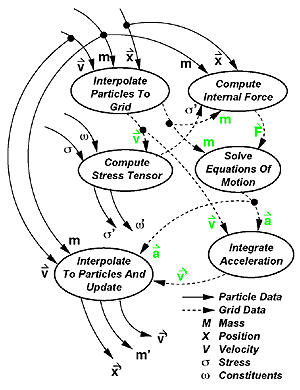
\includegraphics[scale=1]{Taskgraph-diagram.png}
  \caption{Example Task Graph}
  \label{fig:TaskGraph}
\end{figure}

The primary advantage of a component-based approach is that it
facilitates the separate development of simulation algorithms, models,
and infrastructure. Components of the simulation can evolve
independently. The component-based architecture allows pieces of the
system to be implemented in a rudimentary form at first and then
evolve as the technologies mature. Most importantly, Uintah allows the
aspects of parallelism (schedulers, load-balancers, parallel
input/output, and so forth) to evolve independently of the simulation
components. Furthermore, components enable replacement of computation
pieces without complex decision logic in the code itself.

\section{Scheduler and Tasks Overview}

\subsection{Scheduler}
The Scheduler in Uintah is responsible for determining the order of
tasks and ensuring that the correct inter-processor data is made
available when necessary. Each software component passes a set of
tasks to the scheduler. Each task is responsible for computing some
subset of variables, and may require previously computed variables,
possibly from different processors. The scheduler will then compile
this task information into a task graph, and the task graph will
contain a sorted order of tasks, along with any information necessary
to perform inter-process communication via MPI. Then, when the
scheduler is executed, the tasks will execute in the pre-determined
order.

\subsection{Tasks}

A task contains two essential components: a pointer to a function
that performs the actual computations, and the data inputs and
outputs, i.e. the data dependencies required by the function.  When a
task requests a previously computed variable from the data warehouse,
the number of ghost cells are also specified.  The Uintah framework
uses the ghost cell information to excecute inter-process
communication to retrieve the necessary ghost cell data.

An example of a task description is presented showing the essential
features that are commonly used by the application developer when
implementing an algorithm within the Uintah framework.  The task
component is assigned a name and in this particular example, it is
called \texttt{taskexample} and a funtion pointer,
\texttt{\&Example::taskexample}.  Following the instantiation of the
task itself, the dependency information is assigned to the tasks.  In
the following example, the task requires data from the previous
timestep (\texttt{Task::OldDW}) associated with the name
variable1\_label and requires one ghost node
(\texttt{Ghost::AroundNodes,1}) level of information which will be
retrieved from another processor via MPI.  In addition, the task will
compute two new pieces of data each associated with different
variables, i.e. \texttt{variable1\_label}, and
\texttt{variable2\_label}.  Finally, the task is added to the scheduler
component with specifications about what patches and materials are
associated with the actual computation.

\begin{Verbatim}[fontsize=\footnotesize]

Task* task = scinew Task("Example::taskexample",this,
                         &Example::taskexample);
task->requires(Task::OldDW, variable1_label, Ghost::AroundNodes, 1);
task->computes(variable1_label);
task->computes(variable2_label);
sched->addTask(task, level->eachPatch(), sharedState_->allMaterials());

\end{Verbatim}

For more complex problems involving multiple materials and
multi-physics calculations, a subset of the materials may only be used
in the calculation of particular tasks.  The Uintah framework allows
for the independent scheduling and computation of variables associated
with an individual material within a multi-physics calculation.

\section{Programmer Interface to Uintah Components}

Components are the Uintah vernacular for the algorithms that have
been implemented within the Uintah Computational Framework (UCF).
For example, the MPM component is a particle based method for structural
dynamics, the Arches component is a method for simulation of unsteady reacting
flows, etc.  The following describes how these and other components are
incorporated within the UCF.

\subsection{Simulation Component Class Description}

Each Uintah component can be described as a C++ class that is derived
from two other classes: \textbf{UintahParallelComponent} and a
\textbf{SimulationInterface}. The new derived class must provide the
following virtual methods: \texttt{problemSetup},
\texttt{scheduleInitialize}, \texttt{scheduleComputeStableTimestep},
and \texttt{scheduleTimeAdvance}.  Here is an example of the typical
*.h file that needs to be created for a new component.

\begin{Verbatim}[fontsize=\footnotesize]
class Example : public UintahParallelComponent, public SimulationInterface {
  public:

    virtual void problemSetup(const ProblemSpecP& params, 
                              const ProblemSpecP& restart_prob_spec, 
                              GridP& grid, SimulationStateP&);

    virtual void scheduleInitialize(const LevelP& level,SchedulerP& sched);
                                    
    virtual void scheduleComputeStableTimestep(const LevelP& level, 
                                               SchedulerP&);
                                               
    virtual void scheduleTimeAdvance(const LevelP& level, SchedulerP&);

   private:
    Example(const ProcessorGroup* myworld);
    virtual ~Example();


    void initialize(const ProcessorGroup*,
                    const PatchSubset* patches, 
                    const MaterialSubset* matls,
                    DataWarehouse* old_dw, 
                    DataWarehouse* new_dw);
                    
                    
    void computeStableTimestep(const ProcessorGroup*,
                               const PatchSubset* patches,
                               const MaterialSubset* matls,
                               DataWarehouse* old_dw,
                               DataWarehouse* new_dw);
                               
    void timeAdvance(const ProcessorGroup*,
                     const PatchSubset* patches,
                     const MaterialSubset* matls,
                     DataWarehouse* old_dw,
                     DataWarehouse* new_dw);
}
\end{Verbatim}


Each new component inherits from the classes
\textbf{UintahParallelComponent} and \textbf{SimulationInterface}.
The component overrides default implementations of various methods.
The above methods are the essential functions that a new component
must implement.  Additional methods to do AMR will be described as
more complex examples are presented.  Note that in implementing most
algorithms, \tt scheduleTimeAdvance \normalfont actually
schedules several tasks, each of which is responsible for a portion
of the algorithm, rather than scheduling a single \tt timeAdvance \normalfont
task.
The roles of each of the scheduling methods e.g. \texttt{scheduleInitialize},
\texttt{scheduleComputeStableTimestep}, and \texttt{scheduleTimeAdvance}
are described below. 

\subsubsection{ProblemSetup}


The purpose of this method is to read the problem specification (.ups
file (Section~\ref{Sec:UPS})) which
requires a minimum of information about the grid used (e.g. spatial extents,
spatial resolution, patch configuration, etc), time
information, (e.g. time step size, length of time for simulation, etc)
data archiving (e.g., what variables are saved, how frequently, when to
checkpoint for restart, etc).  Depending on the component and the problem
that is being solved, the input file can be rather complex, and this method
would evolve to establish those parameters needed to initially
setup the problem.

\subsubsection{ScheduleInitialize}

The purpose of this method is to initialize the grid data with values
read in from the problemSetup and to define what variables are
actually computed in the TimeAdvance stage of the simulation.  A task
is defined which references a function pointer called
\texttt{initialize}.

\subsubsection{ScheduleComputeStableTimestep}

The purpose of this method is to compute the size of the next timestep in the
simulation.  A task is defined which references a function pointer
called \texttt{computeStableTimestep}.

\subsubsection{ScheduleTimeAdvance}

The purpose of this method is to schedule the actual algorithmic
implementation.  For simple algorithms, there is only one task defined
with a minimal set of data dependencies specified.  However, for more
complicated algorithms, the best way to schedule the algorithm is to
break it down into individual tasks.  Each task of the algorithm will
have its own data dependencies and function pointers that reference
individual computational methods.

\subsection{Data Storage Concepts}

Tasks ``communicate'' with each other through an entity called the
\tt DataWarehouse. \normalfont  The \tt DataWarehouse \normalfont is accessed through a simple
name-based dictionary mechanism and provides each task with the
illusion that all memory is global.  If the tasks correctly describe
their data dependencies, then the data stored in the DataWarehouse
will match the data (variable and region of space) needed by the task.
In other words, the \tt DataWarehouse \normalfont is an abstraction of a global
single-assignment memory, with automatic data lifetime management and
storage reclamation.  Values stored in the \tt DataWarehouse \normalfont are
typically array-structured.

During the course of the simulation, data is computed and stored in
the DataWarehouse.  Data that is from a previous
timestep is stored in the Old DataWarehouse, called \texttt{OldDW},
and data that is computed in the current timestep is stored in the New
DataWarehouse, called \texttt{NewDW}.  At the end of the timestep,
current timestep data is moved to the old data warehouse for the next
timestep in the simulation.


